\begin{lemma}
The points of intersection of \textbf{Line} $L:\vec{x}=\vec{q}+\mu\vec{m}$ with \textbf{parabola}

\begin{align}
\vec{x^T}\vec{V}\vec{x}+2\vec{u^T}\vec{x}+f=0
\end{align}

is given by:
\begin{align}
\vec{x}_i = \vec{q}+\mu_i\vec{m}
\end{align}
%
where,
\begin{multline}
\mu_i = \frac{1}
{
\vec{m}^T\vec{V}\vec{m}
}
\lbrak{-\vec{m}^T\brak{\vec{V}\vec{q}+\vec{u}}}
\\
\pm
{\small
\rbrak{\sqrt{
\sbrak{
\vec{m}^T\brak{\vec{V}\vec{q}+\vec{u}}
}^2
-
\brak
{
\vec{q}^T\vec{V}\vec{q} + 2\vec{u}^T\vec{q} +f
}
\brak{\vec{m}^T\vec{V}\vec{m}}
}
}
}\label{2/37/quad}
\end{multline}
\end{lemma}
\begin{proof}
The points of intersection must satisfy the line and parabola equation.
Thus,
\begin{align}
\vec{\brak{\vec{q}+\mu\vec{m}}^T}\vec{V}\vec{\brak{\vec{q}+ \mu\vec{m}}}+2\vec{u^T}\vec{\brak{\vec{q}+\mu\vec{m}}}+f=0
\end{align}
On expansion, we get
\begin{multline}
  \mu^2\vec{m^T}\vec{V}\vec{m}+ \mu\sbrak{\vec{m^T}\vec{V}\vec{q}+\vec{q^T}\vec{V}\vec{m}+2\vec{u^T}\vec{m}}\\ + \vec{q^T}\vec{V}\vec{q}+2\vec{u^T}\vec{m}+f=0  
\end{multline}
Since, $\vec{q^T}\vec{V}\vec{m},2\vec{u^T}\vec{m}$ are scalars
\begin{align}
 \vec{q^T}\vec{V}\vec{m}=\vec{m^T}\vec{V^T}\vec{q} \\
 2\vec{u^T}\vec{m}=2\vec{m^T}\vec{u}
\end{align}
Solving the above quadratic equation we get
\begin{multline}
\mu_i = \frac{1}
{\vec{m}^T\vec{V}\vec{m}
}\lbrak{-\vec{m}^T\brak{\vec{V}\vec{q}+\vec{u}}}
\\\pm{\small
\rbrak{\sqrt{
\sbrak{
\vec{m}^T\brak{\vec{V}\vec{q}+\vec{u}}
}^2-\brak{\vec{q}^T\vec{V}\vec{q} + 2\vec{u}^T\vec{q} +f
}\brak{\vec{m}^T\vec{V}\vec{m}}
}}}
\end{multline}
\end{proof}
\textbf{First} we consider the parabola $x^2 = 4y$

The matrix parameters of the parabola are
\begin{align}
\vec{V}=\myvec{1&0\\0&0},\vec{u}=\myvec{0\\-2},f=0 \label{2/37/quadform/2/105/eq:v}
\end{align}

Now, we find the points of intersections with the square

The first line is
\begin{align} 
y=4
\end{align}

 The parametric form is:
\begin{align} 
L: \vec{x}&=\vec{q}+\mu\vec{m}
\\
\implies \vec{x}&=\myvec{0\\4}+\mu\myvec{1\\0} \label{2/37/quadform/2/105/eq:q}
\end{align}
From  \eqref{2/37/quad},
\begin{align}
\mu_1 &= 4, \mu_2 =-4
\end{align}
Substituting $\mu_1$ and $\mu_2$ in \eqref{2/37/quadform/2/105/eq:q},the points of intersection
\begin{align}
 \vec{M_1}= \myvec{4\\4},  
\vec{P_1}&= \myvec{-4\\4}
\end{align}

The next line is 
\begin{align} 
y=0
\end{align}
The parametric form is:
\begin{align} 
L: \vec{x}&=\vec{q}+\mu\vec{m}
\\
\implies \vec{x}&=\myvec{0\\0}+\mu\myvec{1\\0} \label{2/37/quadform/2/105/eq:r}
\end{align}
From  \eqref{2/37/quad},
\begin{align}
\mu = 0
\end{align}
Substituting $\mu$ in \eqref{2/37/quadform/2/105/eq:r},the point of intersection
\begin{align}
 \vec{K_1}= \myvec{0\\0}
\end{align}

\textbf{Next} we consider the parabola $y^2 = 4x$

The matrix parameters of the parabola are
\begin{align}
\vec{V}=\myvec{0&0\\0&1},\vec{u}=\myvec{-2\\0},f=0 \label{2/37/quadform/2/105/eq:vi}
\end{align}


The first line is
\begin{align} 
y=4
\end{align}

 The parametric form is:
\begin{align} 
L: \vec{x}&=\vec{q}+\mu\vec{m}
\\
\implies \vec{x}&=\myvec{0\\4}+\mu\myvec{1\\0} \label{2/37/quadform/2/105/eq:qi}
\end{align}
From  \eqref{2/37/quad},
\begin{align}
\mu &= 4
\end{align}
Substituting $\mu$ in \eqref{2/37/quadform/2/105/eq:qi},the points of intersection
\begin{align}
 \vec{M_2}= \myvec{4\\4}
\end{align}

The next line is 
\begin{align} 
y=0
\end{align}
The parametric form is:
\begin{align} 
L: \vec{x}&=\vec{q}+\mu\vec{m}
\\
\implies \vec{x}&=\myvec{0\\0}+\mu\myvec{1\\0} \label{2/37/quadform/2/105/eq:ri}
\end{align}
From  \eqref{2/37/quad},
\begin{align}
\mu = 0
\end{align}
Substituting $\mu$ in \eqref{2/37/quadform/2/105/eq:ri},the point of intersection
\begin{align}
 \vec{K_2}= \myvec{0\\0}
\end{align}

So, both the parabolas intersect each other and the given square at the points 
\begin{align}
 \vec{K}= \myvec{0\\0},
 \vec{M}= \myvec{4\\4}
\end{align}


Area of the square i.e., $A_1$ 
\begin{align}
    A_1 &= Ar(KLMNK)\\
    &= \int_0^4 4dx\\
    &= 16
\end{align}

Area under the parabola $y^2 = 4x$ i.e., $A_2$
\begin{align}
    A_2 &= \int_0^4 \sqrt{4x} dx\\
   &= \frac{1}{6}((16)^{3/2} - 0)\\
   &= \frac{32}{3}
\end{align}

Area under the parabola $x^2 = 4y$ i.e., $A_3$
\begin{align}
    A_3 &= \int_0^4 \frac{x^2}{4}\\
    &= \frac{1}{12}((4)^3 - 0)\\
    &= \frac{16}{3}
\end{align}
As shown in the figure, as the parabolas divide the square into 3 parts

Area of first region is
\begin{align}
    A &= A_1 - A_2\\
    &= 16 - \frac{32}{3} \\
    &= \frac{16}{3}
\end{align}

Area of the second region is
\begin{align}
    B &= A_2 - A_3\\
    &= \frac{32}{3} - \frac{16}{3}\\
    &= \frac{16}{3}
\end{align}

Area of the third region is
\begin{align}
    C &= A_3\\
    &= \frac{16}{3}
\end{align}

So, the 2 parabolas divide the area bounded by the square into 3 equal parts.
\begin{figure}[ht]
\centering
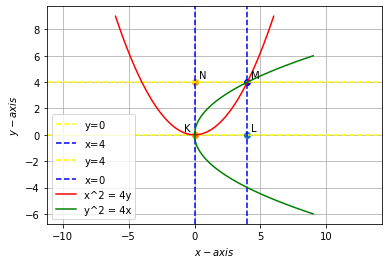
\includegraphics[width=\columnwidth]{solutions/oct/2/37/Figure/AS_5.png}
\caption{plot}
\label{2/37/fig:my_label}
\end{figure}

\begin{tabular}{ |p{2cm}||p{1.5cm}|p{1.5cm}|p{1.5cm}|p{1cm}|p{1cm}|p{1cm}| p{1cm}|p{1.5cm}|p{1.5cm}|}
 \hline
 Parabola & $\vec{V}$ & $\vec{u}$ &$f$&$\vec{q}$ & $\vec{m}$& $\mu_1$ & $\mu_2$& $\vec{POI_1}$ & $\vec{POI_2}$ \\
 \hline
 $x^2 = 4y$   & $\myvec{1 & 0 \\ 0 & 0}$    & $\myvec{0 \\ -2}$ & 0 & $\myvec{0 \\ 4}$ & $\myvec{1 \\ 0}$&4 & -4& $\myvec{4 \\ 4}$ & $\myvec{-4 \\ 4}$\\
 \hline
 $x^2 = 4y$  &   $\myvec{1 & 0 \\ 0 & 0}$ & $\myvec{0 \\ -2}$   &0 & $\myvec{0 \\ 0}$ & $\myvec{1 \\ 0}$& 0 & - & $\myvec{0 \\ 0}$&-\\
 \hline
 $y^2 = 4x$ &$\myvec{0 & 0 \\ 0 & 1}$& $\myvec{-2 \\ 0}$   &0 & $\myvec{0 \\ 4}$  & $\myvec{1 \\ 0}$& 4& - & $\myvec{4 \\ 4}$&-\\
 \hline
 $y^2 = 4x$ &$\myvec{0 & 0 \\ 0 & 1}$& $\myvec{-2 \\ 0}$    &0  & $\myvec{0 \\ 0}$  & $\myvec{1 \\ 0}$& 0& - & $\myvec{0 \\ 0}$&-\\
 
 \hline
\end{tabular}
